\subsubsection{Recursion}
\label{section:perf-recursion}

The next question to explore is the performance characteristics of the SUTs when executing a recursion heavy program. To begin, we will look at the \texttt{fibonacci(n)} test suite. At first glance, this will seem very similar to the \texttt{primal(n)} test suite: as \texttt{n} increases the program hotness will increase. The fact that \texttt{fibonacci(n)} is recursive has some important implications.

Firstly, the proportion of memory instructions will be much higher. As memory operations are required for the stack, the program will have a lower arithmetic intensity. Secondly, the recursive function must use \texttt{JR} to unwind the stack, a variable jump that cannot be relinked by \texttt{-L} as explained in \autoref{section:direct-linking}. These factors will help us determine which aspects of the performance characteristics observed previously were due to program hotness, and what was due to arithmetic intensity.

\YIComment{Redo this}

\autoref{figure:fibonacci-mips} shows the performance of the \texttt{fibonacci(n)} test suite. It has a very similar performance characteristic to the \texttt{primal(n)} test suite with some notable differences.

The overall performance for both SUTs is significantly lower. This is due to the memory instructions required for pushing and popping the stack, which have much lower emulation performance compared to arithmetic instructions.

The JIT emulator takes significantly longer to reach peak performance whereas the interpreter does not. This is because the interpreters fixed costs, such as initialization, do not change with the program being executed. The JIT emulator on the other hand has additional costs for every block that needs compiling, and the \texttt{fibonacci(n)} program contains more source blocks. This means there is a larger initial cost which takes longer to amortize.

\begin{figure}[H]
    \centering
    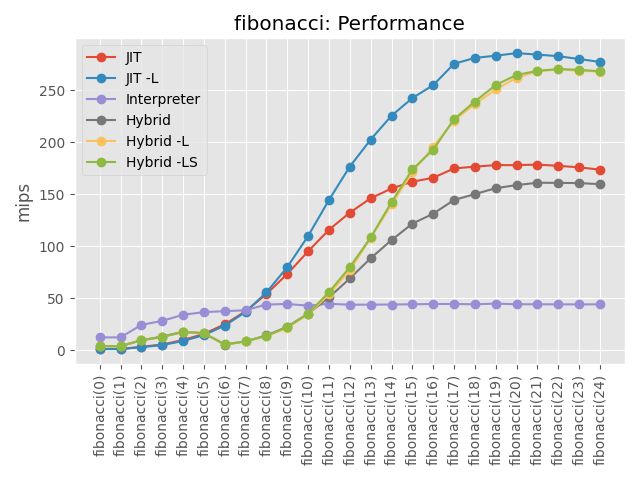
\includegraphics[scale=0.75]{output/graphs/tests/all/fibonacci/mips.png}
    \caption{Performance in mips of the fibonacci test suite.}
    \label{figure:fibonacci-mips}
\end{figure}

\YIComment{Talk about factorial}

\begin{figure}[H]
    \centering
    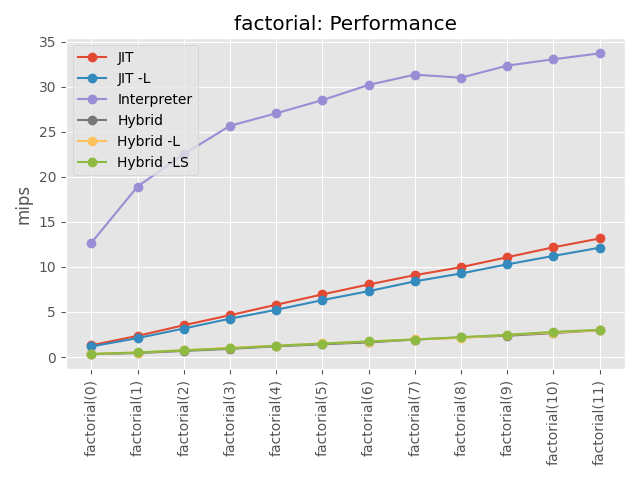
\includegraphics[scale=0.75]{output/graphs/tests/all/factorial/mips.png}
    \caption{Performance in mips of the factorial test suite.}
    \label{figure:factorial-mips}
\end{figure}